\documentclass[a4paper,12pt,twoside]{report}
\usepackage[english]{babel}
\usepackage[utf8]{inputenc}
\usepackage{amsmath}
\usepackage{amssymb}
\usepackage{etoc}
\usepackage{layout}
\usepackage{url}
\usepackage{array}
\usepackage{multirow}
\usepackage{float}
\usepackage[backend=bibtex,style=numeric-comp]{biblatex}
\usepackage{tikz}
\usetikzlibrary{automata,positioning}


\usepackage{style} % Local package.

\bibliography{bib/references.bib}

\begin{document}
\begin{titlepage}
\noindent \titlefont Implementation of \\
omega-automata \\
simplification \\
techniques in "Spot", \\
a model checking library.\par
\epigraph{When "Spot" SAT-based minimization meets incremental solving.}%
{\textit{Paris, January 2017}}
\null\vfill
\vspace*{1cm}
\noindent
\hfill%
%
\noindent\begin{minipage}{0.7\textwidth}
    \begin{flushright}
        \printauthor
    \end{flushright}
\end{minipage}%
%
\begin{minipage}{0.1\linewidth}%
  \hspace{0.5cm}%
  \rule{5pt}{200pt}%
\end{minipage}%
%
\begin{minipage}{0.3\textwidth}% adapt widths of minipages to your needs
  
\includegraphics[width=\linewidth]{./img/epita.png} \\%
  \begin{center}%
    
\includegraphics[width=2cm]{./img/spot.png}%
  \end{center}%
  
\includegraphics[width=\linewidth]{./img/lrde.png}%
\end{minipage}%
%
\titlepagedecoration
%
\end{titlepage}%			Title page.
\etocdepthtag.toc{mtchapter}
\etocsettagdepth{mtchapter}{subsection}
\etocsettagdepth{mtappendix}{none}
\tableofcontents
\addtocontents{toc}{\protect\thispagestyle{empty}}%		First table of contents.

\part{Report}
\chapter{LRDE Presentation}


\section{Line of business}
The \LRDE\space (Research and Development Laboratory of \EPITA) is focused on fundamental
research and development in computer science. Its main areas of expertise are:
\begin{itemize}
 \item Image processing and pattern recognition
 \item Automata and verification
 \item Performance and genericity
\end{itemize}


\noindent Building on its solid scientific production and academic collaborations, the laboratory has
industrial contracts, conducts internal research projects and participates in collaborative
academic research projects.

\noindent Its members also give classes to students at \EPITA\space from the first year of engineering.

\section{The Laboratory}
The \LRDE\space (\url{https://www.lrde.epita.fr/wiki/Home}) was created in February 1998 to promote
the research activity at \EPITA\space and to allow students to be involved into important research
projects.

The research activity at \LRDE\space is focusing on subjects related to the school with the aim
of getting recognition in the scientific domain through publications and by working together with other
research centers.\\
One particularity of the \LRDE\space is the will to create a bond between traditional
teaching given to \EPITA\space students and teaching through research. The point of this is to:
\begin{itemize}
  \item participate to the production of knowledge in computer science and to
	promote the image of \EPITA\space in scientific domain.
  \item develop \LRDE\space student's formation through research and allow them to access a third cycle
	formation.
\end{itemize}


\section{Members}
The laboratory is currently composed of thirteen permanent members, including teacher-researchers, engineers
and administration.

\noindent In addition to permanent staff, the \LRDE\space also hosts PhD students. Currently, there are five
of them. During the whole duration of their doctoral studies, they work with two advisor researchers, one of
the \LRDE\space and one of another university (joint supervision in partnership).

Each year, the permanent members recruit third year students from \EPITA, whom will stay until the
end of their studies, following a dedicated study specialisation at \EPITA\space. Hence, the laboratory
hosts two generations of students that can grow to a number between ten to fifteen.


\section{Services}
The \LRDE\space is working on four different axis:


\subsection{Image Processing}
\subsubsection{Olena}
\begin{center}
 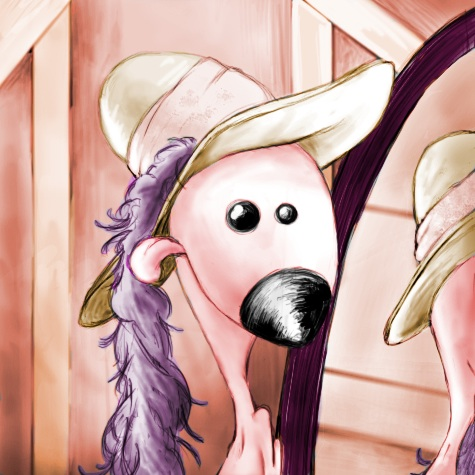
\includegraphics[width=2cm]{img/olena.jpg}
\end{center}
The Olena project (\url{https://olena.lrde.epita.fr}) consists of a generic image processing library.
Its objective is to implement a platform of numerical scientific computations dedicated to image
processing, pattern recognition and computer vision. This environment is composed of a generic and
efficient library (Milena), a set of tools for shell scripts and a visual programming interface.
The project aims at offering an interpreted environment like MatLab or Mathematica. It provides many
ready-to-use image data structures (regular 1D, 2D, 3D images, graph-based images, etc.) and algorithms.
Milena's algorithms are built upon classical entities from the image processing field (images, points/sites,
domains, neighborhoods, etc.).\\

Each of these parts imply its own difficulties and require the development of new solutions.
For example, the library, which require the entirety of low level features on which it relies on to be
both efficient and generic --- two objectives that are hard to meet at the same time in programmation.
Fortunately, the object oriented programming eases this problem if we avoid the classical object
modeling with inheritance and polymorphism. Hence, this genericity allows the development of efficient
and re-usable code - i.e. developers or practitioners can easily understand, modify, develop and extend
new algorithms while retaining the core traits of Milena: genericity and efficiency.
The Olena platform uses this paradigm. The project already addressed the problem of the diversity of data
and data structures.\\

Furthermore, the people working on this project were able to put in light the existence of conception
models related to generic programmation. Olena is an open source project under General Public License (GPL)
version 2.


\subsubsection{Climb}
The Climb team of the laboratory has chosen to focus on the persistent question of performance and
genericity, only from a different point of view.\\

The purpose of this research is to examine the solutions offered by languages other than C++, dynamic
languages notably, and Lisp in particular. C++ has its drawbacks, it is a heavy language with an extremely
complex and ambiguous syntax, the template system is actually a completely different language from standard
C++ and finally it is a static language. This last point has significant implications on the application,
insofar as it imposes a strict chain of Compilation $\rightarrow$ Development $\rightarrow$ Run
$\rightarrow$ Debug, making for example rapid prototyping or human-machine interfacing activities difficult.
It becomes therefore essential to equip the involved projects with a third language infrastructure that is
rather based on scripting languages.\\

The Climb project aims at investigating the same domain as Olena, but starting from an opposite view.
It express the same issues following an axis of dynamic genericity and compares the performance obtained by
some Common Lisp compilers with those of equivalent programs written in C or C++.

\subsection{Finite state machine manipulation}
\subsubsection{\VCSN}
\begin{center}
 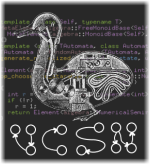
\includegraphics[width=2cm]{img/vcsn.png}
\end{center}
The \VCSN project (\url{https://vcsn.lrde.epita.fr}) is a finite state machine manipulation
platform developed in collaboration with the ENST. Finite state machines, also called automata,
are useful for language treatment and task automation. In the past, such platforms, like "FSM",
were supposed to work for problems of industrial scale. Hence, for efficiency reasons, they were
specialized in letter automata. On the other hand, platforms like "FSA" were based on a more abstract
approach. \VCSN tries to answer both of these issues by using techniques of static and generic
programmation in C++.\\

\VCSN can then support the entirety of automata with multiplicity in any kind of
semiring. Thanks to generic programming techniques, it is not necessary to code a single algorithm once
for each type of automata anymore. A single abstract version is sufficient, and this without loosing
efficiency. It is not necessary to handle C++ perfectly to be able to use the platform thanks to an
interpreter conceived to highlight all of the system's potential. This environment should allow
researchers to experiment their ideas and beginners to practice with an intuitive interface.\\

\VCSN is an open source project under GPL license.


\subsection{Model checking}
\subsubsection{Spot}
\begin{center}
 
\includegraphics[width=2cm]{img/spot.png}
\end{center}
Spot (\url{https://spot.lrde.epita.fr/}) is a library of algorithms for "model checking",
which is a way to check that every possible behavior of a system satisy its given properties.
Spot allows to express those properties using linear-time temporal logic (LTL). It corresponds to classical
propositional calculus (with its "or", "and" and "not" operators) equiped with temporal operators to
express things such as "in a future time" or "anytime since now". Spot also supports arbitrary 
acceptance condition, transition-based acceptance and four different representation formats of
$\omega$-automata (HOA, never claims, LBTT, DSTAR). All those terms will be explained in the 'basic
concepts' section.\\

Such formulas seen above (LTL formulas) can be translated to automata (Spot implements different algorithms)
, such that verifying that the behavior of a model satisfy a formula can be reduced to operations between
two automata (here again Spot implements different algorithms). This approach can be applied to different kind of systems: communication protocoles,
electronic circuits, programs...\\

This project was born in the MoVe team at LIP6, but since 2007 it is mainly developped by the LRDE, with some
occasional collaborations with LIP6. It is distributed under a GNU GPL version 3 license. 


\subsection{Speaker recognition}
\subsubsection{Speaker ID}
The Speaker Recognition team is working on Machine Learning solutions applied to Speaker Recognition
tasks. They propose statistical representations of speech signal which are more robust to the problem
of session and channel variabilities.\\

A speaker must always be identified, whether he is ill, suffering from sore throats, or his
current emotions bring change to his voice. To do this, all the characteristics of a voice that can change
depending on any external parameter must be ignored. This is one of the issues the Speaker ID team is
facing.\\

They participated in the evaluation campaign of speaker verification systems organized by NIST
(the National Institute of Standards and Technology) which organizes competitions in various fields, both
to stimulate research and to define new standards since the beginning of the project.\\

The work of LRDE Speaker ID team is conducted in collaboration with the Spoken Language Systems Group of
the MIT Computer Science and Artificial Intelligence Laboratory (\url{http://groups.csail.mit.edu/sls/}).


\section{The internship in the company's work}
This internship took place within the team of model checking. It was essentially focused on
the improvement of the SAT-based minimization of $\omega$-automata. This feature is a result of
previous work conducted by \textit{Alexandre Duret-Lutz} and \textit{Souheib Baarir} explained in two
publications (\cite{14} and \cite{15}).%				LRDE description.
\chapter{Spot}
Spot was first presented in 2004~\cite{2}. It was purely a library until Spot 1.0~\cite{1}, when
command-line tools for LTL manipulation and translation of LTL to some generalizations of Büchi Automata
have started to be distributed. Today, Spot 2.0~\cite{25} supports more tools with arbitrary acceptance
conditions as described in the Hanoi Omega Automata format (HOA)~\cite{3} and python bindings usable in
interactive environments such as IPython/Jupyter~\cite{4}.

\section{Structure}
The Spot project can be broken down into several parts, as shown in Figure~\ref{fig:arch}. Orange boxes
are C/C++ libraries. Red boxes are command-line program. Blue boxes are Python-related.
\begin{figure}[H]
 \centering
 \begin{tikzpicture}
  \tikzset{cppbox/.style={minimum width=#1,fill=orange!30, minimum height=1.5cm},
           pybox/.style={minimum width=#1,fill=cyan!30, minimum height=1cm},
           shbox/.style={minimum width=#1,fill=red!30, minimum height=8mm},
           usedby/.style={->,ultra thick,>={Stealth[length=5mm,round]},gray!50!black}}
  \node[cppbox=7.3cm] (libspot) {\texttt{libspot\strut}};
  \node[cppbox=4.3cm,right=2mm]
     (libltsmin) at (libspot.east) {\texttt{libspot-ltsmin\strut}};
  \node[cppbox=8cm,below right,yshift=-2mm,minimum height=8mm] (buddy) at (libspot.south west) {\texttt{libbddx\strut}};

  \node[pybox=4.3cm,above=2mm] (pyltsmin) at (libltsmin.north) {\texttt{import spot.ltsmin\strut}};
  \node[pybox=3cm,left=2mm] (pyspot) at (pyltsmin.west) {\texttt{import spot\strut}};
  \node[shbox=4.1cm,above left,xshift=-2mm,align=center] (shcmd) at (pyspot.south west) {
    \texttt{randltl}\\
    \texttt{genltl}\\
    \texttt{ltlfilt}\\
    \texttt{randaut}\\
    \texttt{autfilt}\\
    \texttt{ltl2tgba}\\
    \texttt{ltl2tgta}\\
    \texttt{dstar2tgba}\\
    \texttt{ltlcross}\\
    \texttt{ltlgrind}\\
    \texttt{ltldo}
  };
  \node[shbox=1.9cm,below left,yshift=-2mm] (divine) at (libltsmin.south east) {\texttt{divine\strut}};
  \node[shbox=1.5cm,left,xshift=-2mm] (spins) at (divine.west) {\texttt{SpinS\strut}};
  \node[pybox=7.5cm,above right,yshift=2mm] (ipython) at (pyspot.north west) {IPython / Jupyter};
  \draw[usedby] (buddy.north) -- ++(0,3mm);
  \draw[usedby] (buddy.north) ++(3.7cm,0) -- ++(0,3mm);
  \draw[usedby] (spins.north) -- ++(0,3mm);
  \draw[usedby] (divine.north) -- ++(0,3mm);
  \draw[usedby] (libspot.east) -- ++(3mm,0);
  \draw[usedby] (pyspot.south) ++(0,-2mm) -- ++(0,3mm);
  \draw[usedby] (pyltsmin.south) ++(0,-2mm) -- ++(0,3mm);
  \draw[usedby] (shcmd.south) ++(0,-2mm) -- ++(0,3mm);
  \draw[usedby] (pyspot.north) -- ++(0,3mm);
  \draw[usedby] (pyltsmin.north) -- ++(0,3mm);

  \begin{pgfonlayer}{background}
  \path[fill=gray!15,draw=gray,rounded corners=1mm]
  ($(shcmd.north west)+(-1mm,1mm)$) --
  ($(shcmd.north east)+(1mm,1mm)$) --
  ($(pyspot.north west)+(-1mm,1mm)$) --
  ($(pyltsmin.north east)+(1mm,1mm)$) --
  ($(libltsmin.south east)+(1mm,-1mm)$) --
  ($(buddy.north east)+(1mm,1mm)$) --
  ($(buddy.south east)+(1mm,-1mm)$) --
  ($(buddy.south west)+(-1mm,-1mm)$) -- cycle;
  \end{pgfonlayer}
\end{tikzpicture}
 %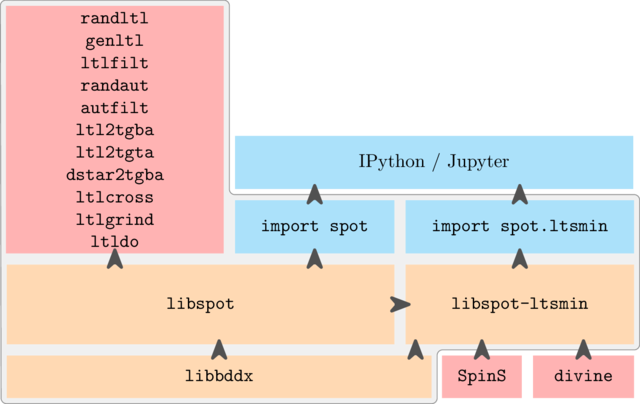
\includegraphics[scale=0.6]{img/arch.png}
 \caption{Architecture of Spot}
 \label{fig:arch}
\end{figure}
Spot is actually split in three libraries:
\begin{itemize}
 \item libbddx is a customized version of BuDDy for representing Binary Decision Diagrams which we use to
label transitions in automata, and to implement a few algorithms.
 \item libspot is the main library containing all data structures and algorithms.
 \item libspot-ltsmin contains code to interface with state-spaces generated as shared libraries by LTSmin.
\end{itemize}


\section{Command-line tools}
Spot 2.0 installs the following eleven command-line tools, that are designed to be combined as traditional
Unix tools.\\
\begin{figure}[H]
 \begin{tabular}{l c | m{8cm}}
  \multirow{13}{*}{SPOT 1.0~\cite{1}}&randltl&Generates random LTL/PSL formulas\\
   &genltl&Generates LTL formulas from scalable patterns\\
   &ltlfilt&Filter, converts, and transforms LTL/PSL formulas\\
   &ltl2tgba&Translates LTL/PSL formulas into generalized Büchi automata~\cite{7}, or deterministic parity
	     automata (new in 2.0)\\
   &ltl2tgta&Translates LTL/PSL formulas into Testing automata~\cite{6}\\
   &ltlcross&Cross-compares LTL/PSL-to-automata translators to find bugs (works with arbitrary acceptance
	     conditions since Spot 2.0)\\
   \hline
   &ltlgrind&mutates LTL/PSL formulas to help to reproduce bugs on smaller ones\\
   &dstar2tgba&converts ltl2dstar automata into Generalized Büchi automata~\cite{14}\\
   &randaut&generates random $\omega$-automata\\
   &autfilt&filters, converts and transforms $\omega$-automata\\
   &ltldo&runs LTL/PSL formulas through other translators, providing uniform input and output interfaces\\
 \end{tabular}
 \caption{Spot tools description}
\end{figure}

\section{The Python Interface}
Similar tasks can be performed in a more ''algorithm-friendly'' environment using the Python interface.
Combined with the IPython/Jupyter notebook~\cite{4} (a web application for interactive programming), this
provides a nice environment for experiments, where automata and formulas are automatically displayed.

\section{Workflow}
Working on any project of the LRDE implies to follow some rules. That allows a better integration of each
member. Once a patch is ready, any member of the model checking team can reread the patch and make
suggestions.

\subsection{Coding conventions}
As Spot is a free software, uniformity of the code matters a lot. Some coding conventions are used so that
the code looks homogeneous. Here are some points:
\begin{itemize}
 \item UTF-8 is used for non-ASCII characters.
 \item tabs are not used for indentation in files, only spaces, in order to prevent issues with people
 assuming different tab widths.
 \item \#include with angle-brackets refers to public Spot headers (i.e those that will be installed, or
 system headers that have already been installed).
 \item \# include with double quotes refer to private headers that are distributed with Spot.
\end{itemize}

Have a look at \url{https://gitlab.lrde.epita.fr/spot/spot/blob/master/HACKING} for more details

\subsection{Git Versionning Tool}
The versionning tool used in Spot is Git. All development branches except 'master' and 'next' follows a
particular naming convention: \{initials\}/\{subject of work\}. This allows a quick glance to identify
who works on which branch and on what.

Concerning commits, large commits introducing a feature are preferred to many small commits covering
the same feature. Suppose that a new feature must be implemented and needs 3 key steps. Even if each step
is done in many commits during the development, at the end, it's better to squash commits so as to have
only 3 large commits representing the 3 key steps.

Also, if at any moment in turns out that a previous work
could have been done otherwise, any update must be applied directly to the commit concerned --- each commit
must actually insert code in its final form.

\subsection{Adding Tests}
Any implementation done must be tested and any feature should be documented. For the purpose on one hand
to avoid regression and on the other hand to ensure the code runs as expected. All tests are located in
the 'tests' folders. Most of them are written in Python (using the python bindings) or shell script.

%				SPOT description.
\chapter{Basic concepts}%			Basic concepts definitions.
\chapter{Contributions to Spot}

This chapter present the different things I have done on Spot during the internship. Might it be
some algorithms implemented, scripts, display arrangements, benchmarks, results analyzes, etc.

\noindent All the achieved work is presented in a chronological way, to bring out the difficulties
encountered, the unexpected results that had influence on the advancement of the work.

\section{fastSAT}
As a quick reminder, here are the required characteristics for the SAT solver:
\begin{itemize}
 \item licence compatibility with Spot's one (GNU GPL v3),
 \item simplicity of integration for future updates,
 \item effectiveness.
\end{itemize}

\noindent The project \textbf{fastSAT}\cite{5} was born to help choose the SAT solver to distribute with
Spot. Until now, SAT-based minimization was performed through an external SAT solver. The default one
was Glucose \cite{12} (3.0 version). Therefore, it seems logical to consider Glucose as a possible
candidate. \textbf{fastSAT}\cite{5} compared Glucose 4.0 \cite{12} to CryptoMiniSat 5.0.1\cite{20} and
PicoSAT 965 \cite{21}. Note that some SAT solvers provide two versions, one parallal and one simple
essentially because of the SAT competitions. In short, were compared:
\begin{itemize}
 \item Glucose syrup (parallal) 4.0
 \item Glucose simple 4.0
 \item CryptoMiniSat parallal 5.0.1
 \item CryptoMiniSat simple 5.0.1
 \item PicoSAT 965
\end{itemize}

The next three figures (\ref{fig:satchoose_1}, \ref{fig:satchoose_2} and \ref{fig:satchoose_3}) show some
comparaisons for three formulas. About twenty formulas have been tested in two modes: by forcing the number
of state and by doing the complete cycles of minimization. It has been executed on a computer with an
\textbf{Intel(R) Core(TM) i7-4710HQ CPU @ 2.50GHz} processor and  a \textbf{8 GiB} system memory.
The measuring tool used is the open Google Benchmark tool \cite{22}.

\begin{figure}[H]
 \centering
 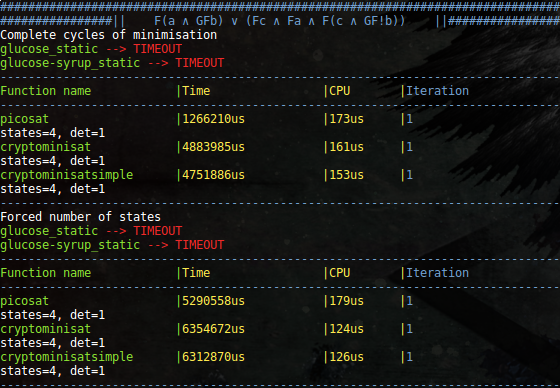
\includegraphics[scale=0.7]{img/satchoose_1.png}
 \caption{Benchmark for formula $F(a \land GFb) \lor (Fc \land Fa \land F(c \land GF(!b)))$}
 \label{fig:satchoose_1}
\end{figure}

\begin{figure}[H]
 \centering
 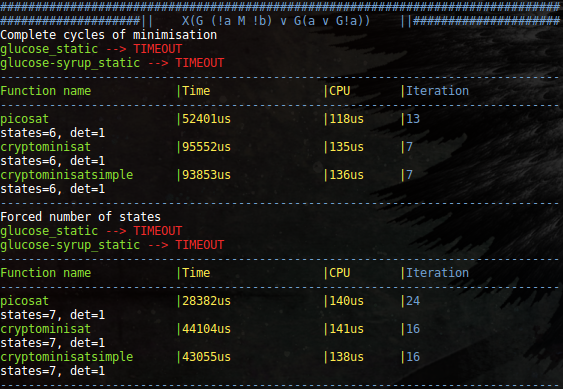
\includegraphics[scale=0.7]{img/satchoose_2.png}
 \caption{Benchmark for formula $X(G (!a M !b) \lor G(a \lor G(!a)))$}
 \label{fig:satchoose_2}
\end{figure}

\begin{figure}[H]
 \centering
 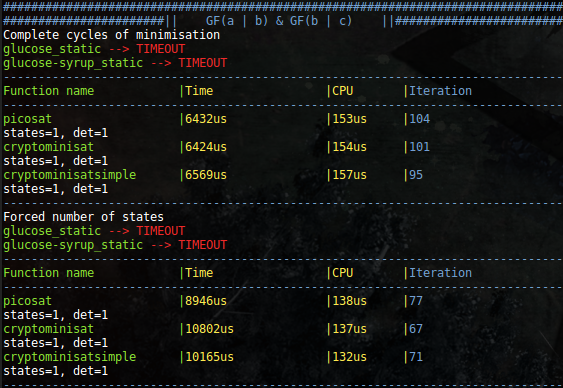
\includegraphics[scale=0.7]{img/satchoose_3.png}
 \caption{Benchmark for formula $GF(a \lor b) \land GF(b \lor c)$}
 \label{fig:satchoose_3}
\end{figure}

\noindent In conclusion, among the different SAT solvers, \textbf{PicoSAT} was choosen for its strong
performances. It consists of two source code files: \textbf{picosat.h} and \textbf{picosat.c} and was
easily integrated and harmonised with Spot.

\textbf{fastSAT}\cite{5} project is fully availlable and anyone can reproduce the benchmarks. Feel free to
have a look.

\section{New Satsolver class}
There was already a satsolver class that is instantiated at the beginning of the SAT-based minimization
procedures, formerly used to initialize a temporary \textbf{cnf file} (DIMACS \cite{18}), return
it and call the external SAT solver. The file writing was directly made by those procedures.

\noindent The objective is to completely abstract the file writing. SAT-based minimization procedures will
just have to instantiate a satsolver object at the beginning and make calls to its functions. Thoses
functions will call the SAT solving library functions. But this class must continue to support any external
SAT solver by handling temporary \textbf{cnf files}.\\

\begin{figure}[h]
  \centering
  \begin{tikzpicture}
    \begin{umlpackage}{Pseudo UML}
     \umlclass[name=satsolver, template=T]{spot::satsolver}
     {
       psat\_ : PicoSAT*\\
       cnf\_stream\_ : std::ostream*\\
       nb\_clauses\_ : int\\
       nb\_vars\_ : int\\
       ...
       }{
       add(std::initializer\_list\textless int\textgreater values : void\\
       add(int v) : void\\
       comment(T first, Args... args)\\
       get\_nb\_clauses() : int\\
       get\_nb\_vars() : int\\
       get\_solution() : std::pair\textless int, std::vector\textless bool\textgreater\textgreater\\
       ...
     }
    \end{umlpackage}
  \end{tikzpicture}
  \caption{Satsolver class UML representation}
  \label{fig:sat_uml}
\end{figure}

\noindent The figure \ref{fig:sat_uml} shows an approximate UML representation of the new satsolver class.
It can either initialize PicoSAT or a cnf\_stream\_. The idea is to let its functions (add, comment, etc.)
to decide if they call PicoSAT functions or write in the cnf\_stream\_. That way, SAT-based minimization
procedures are not aware of what's going on behind and can repeat over and over again the same algorithms.\\

\noindent Of course the clause counting mechanism is provided by the new satsolver class. At the end,
SAT-based procedures will just have to call the \textit{get\_solution()} method.\\

Once this was done, SAT-based procedures had already gained some speed which is entirely understandable as
disk operations are slow. For instance, with this command
line:
\begin{lstlisting}[language=bash,caption={bash command-line to test a formula minimization using ltl2tgba}]
  time ltl2tgba -D -x sat-minimize 'G(a -> Fb) & G(c -> Fd)'
                        --stats='states=%s, det=%d'
\end{lstlisting}
This result is obtained on a Macbook pro with \textbf{2,9GHz intel core i5} and
\textbf{8 Go 1867 Mhz DDR3}:\\\\
\begin{tabular}{|c|c|}
 \hline
 &\\
 PicoSAT as & Time result\\
 &\\
 \hline
 &\\
 linked SAT solving library&0.29s user 0.08s system 98\% cpu 0.371 total\\
 external SAT solver (with disk operations)&0.82s user 0.09s system 98\% cpu 0.925 total\\
 &\\
 \hline
\end{tabular}

\section{First incremental approach}
\label{approach1}
Just as a reminder, until now, SAT-based minimization procedures whether it is with binary search
(algorithm \ref{dicho}) or the naive way (algorithm \ref{naive}), starts the SAT encoding from scratch
at each step of the cycle of minimization; that is unfortunate. This is why an incremental approach
has been considered.\\

\noindent  The algorithm \ref{incr1} has been implemented. Starting with an $\omega$-automaton of size
$n$, if the first iteration (which encodes the research of an $\omega$-automaton of size $n-1$) constructs
an automaton of $k$ ($k \leq n-1$) states \textit{accessible}, then some clauses are added to forbid all the
entrant transitions of the $n-k-1$ last state. If such automaton is found, the entrant transitions of the
$n-k-2$ last state are also forbidden, etc. The last SAT problem solved correspond to the minimal
automaton.\\

\noindent An interesting thing, as a sideline, is that at the beginning, instead of forbidding the entrant
transitions of a state, the outgoing transitions were forbidden. This did not work, because those
clauses were in contradiction with the first rule of the encoding (which stated that the automaton must be
\textit{complete}), causing an absurdity. All the rules of the encoding are described in the papers
\cite{14} and \cite{15}.\\

\noindent After this method has been implemented (algorithm \ref{incr1}), a benchmark has been realized to
compare it to the old default method (algorithm \ref{naive}). For dispay reasons, only a few interesting
lines of the results are displayed in the figure \ref{fig:glu_vs_incr1_short}. Feel free to have a look
in the \ref{glu_vs_incr1_complete} section of the appendix to see all the results. For each version and
each formula, two minimizations are attempted, büchi \textit{acceptance set} and
\textit{generalized büchi acceptance set}. The best performances for each formula are colorized
respectively in green and yellow.

\begin{figure}[H]
 \centering
 \fontsize{9}{11}\selectfont{
 \setlength\LTleft{0pt}% default: \parindent
 \setlength\LTright{0pt}% default: \fill
 \begin{longtable}{@{\extracolsep{\fill}}|*{5}{c|}}
  \hline
  \multirow{3}{*}{Formulas}&\multicolumn{4}{c|}{Time (seconds)}\\
  &\multicolumn{2}{c|}{Glucose (As before)}&\multicolumn{2}{c|}{Incr Naive}\\
  &minDBA&minDTGBA&minDBA&minDTGBA\\
  \hline
  $F(a \land  GFb) \lor  (Fc \land  Fa \land  F(c \land  GF\bar b))$&0.02&\cellcolor{Yelw} 57.65&\cellcolor{Green} 0.01&236.36\\
  $XXG(Fa U Xb)$&25.15&\cellcolor{Yelw} 762.74&\cellcolor{Green} 20.21&(killed)\\
  $(a R (b R Fc)) W XGb$&(killed)&\cellcolor{Yelw} 254.19&(killed)&672.80\\
  $X(\bar a \land  Fa) R (a M Fb)$&2.19&\cellcolor{Yelw} 46.12&\cellcolor{Green} 1.7&132.02\\
  $(a R Fb) U X\bar c$&(killed , $\le$ 11)&\cellcolor{Yelw} 389.87&(killed , $\le$ 11)&616.70\\
  \hline
 \end{longtable}}
 \caption{Parts of \ref{glu_vs_incr1_complete} benchmark results showing some cases where the Old SAT-based
          minimization is still better}
 \label{fig:glu_vs_incr1_short}
\end{figure}

In all the lines of the figure \ref{fig:glu_vs_incr1_short}, \textbf{glucose} is still better than our first
incremental approach. There is even a case where \textbf{naive incr} never ends the minimization and
is killed.

In order to better compare both version, this generated figure counts the number of times a version is
better than the other with a tolerance of more or less five percents (5\%). That means: roughly equal times
are skipped.
\begin{figure}[H]
 \centering
 \begin{tabular}{|c|c|c|c|}
\hline
\multicolumn{4}{|c|}{DBA}\\
\hline
&glu&incr1&total\\
\hline
glu&{-}&9&9\\
\hline
incr1&102&{-}&102\\
\hline
\multicolumn{4}{c}{}\\
\hline
\multicolumn{4}{|c|}{DTGBA}\\
\hline
&glu&incr1&total\\
\hline
glu&{-}&8&8\\
\hline
incr1&93&{-}&93\\
\hline
\end{tabular}
 \caption{Summary of \ref{glu_vs_incr1_complete} benchmark}
 \label{fig:glu_vs_incr1_resume}
\end{figure}

The next two figures (\ref{fig:glu_vs_incr1_dba} and \ref{fig:glu_vs_incr1_dtgba}) shows two graphs generated
with ggplot2 \cite{23} (a graphing package implemented in top of the \textbf{R} statistical package). Any
point between the two lines passing through the origin is in the tolerance area (more or less 5\%). All the
bothering points (cases where glucose win) are located in the area over both lines. Obvisouly, the
first incremental approach wins when points are located under both lines.

\begin{figure}[H]
 \centering
 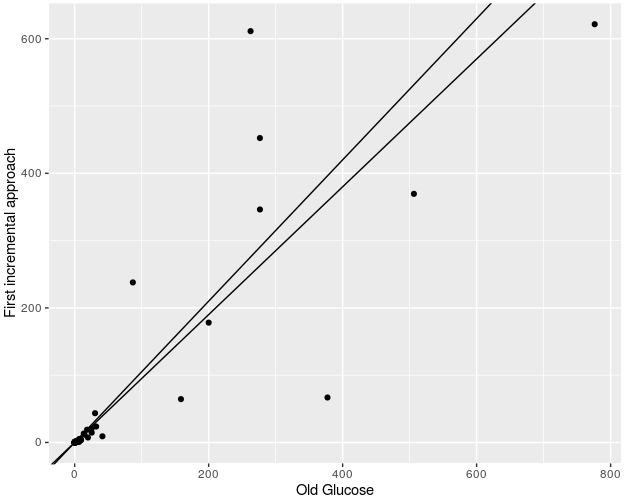
\includegraphics[scale=0.6]{img/glu_vs_incr1_dba.png}
 \caption{Graph comparing both minDBA time of minimization}
 \label{fig:glu_vs_incr1_dba}
\end{figure}

\begin{figure}[H]
 \centering
 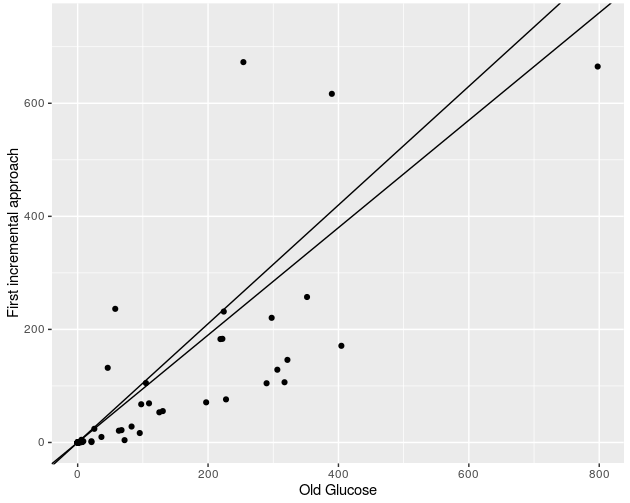
\includegraphics[scale=0.6]{img/glu_vs_incr1_dtgba.png}
 \caption{Graph comparing both minDTGBA time of minimization}
 \label{fig:glu_vs_incr1_dtgba}
\end{figure}

\noindent In light of the above, this incremental approach does not seem to be the most appropriate method.
This is really surprising. Why all that the SAT solver learned while solving the first traditional encoding
did not help him to solve quickly the next similar problems?\\

An hypothesis raised is that may be the fact that the size of the problem is never decreased affect it? By
restarting the encoding from scratch at each step, the Old SAT-based minimization also restarts with a
smaller automaton. The smaller the input automaton is, the smaller the SAT problem produced is (with a
decreasing number of litterals and clauses).\\

As SAT competitions also compares SAT solvers in incremental mode, they have defined a file format,
called XCNF. As our incremental scenarios seem to offer challenges to SAT solver, we decided to provide
a way to generate XCNF file corresponding to complete cycles of this first incremental minimization. We thus
hope that SAT solvers contributors will think about how to improve their solver to be efficient in
these incremental SAT solving scenarios.

\section{A not total incremental approach}
\label{approach2}
With a view to verify the last hypothesis, a similar approach has been proposed.
The idea is to provide the opportunity to choose how many times SAT-based
minimization should work incrementally before restarting the encoding from scratch. Here times can be seen
in two ways. It can be either the number of states to reduce or just a number of attemps before
restarting the encoding. The second way has been chosen because gaining many states when only one is
expected is unpredictable.\\

Here is how the algorithm looks like ($s$ means sat\_incr\_steps and stands for the number of attempts).

\begin{algorithm}[H]
 \caption{This incremental approach attemps a traditional encoding and then tries to exclude
          $s$ states incrementally before restarting the encoding from scratch.}
 \label{incr2}
 \begin{algorithmic}[1]
  \Procedure{\textsc{ReduceStatesDTGBA}$(R,m=R$.nb\_acc\_sets()$, s)$}{}
   \BState \emph{repeat}:
   \State{$n \gets R.nb\_states() $}
   \State{$C \gets \textsc{Synthetize}DTGBA(R,n-1,m) $}
   \If{$C$ \textbf{does not exists}} \Return $R$\EndIf
   \For{$i = 0$; $i < s;$ ++$i$}
    \State{add clauses to exclude one more state}
    \State{$C \gets$ Try to solve the new problem and build the new automaton}
    \If{$C$ \textbf{does not exists}} \Return $R$\EndIf
    \State{$R \gets C$}
   \EndFor
  \EndProcedure
 \end{algorithmic}
\end{algorithm}

Again, once this was implemented, a new benchmark was made. Different values for $s$ has been tested:
$1, 2, 4$ and $8$, $2$ was the best value between them. Again, for some display reasons, only this version
is displayed in comparaison to the Old SAT-based minimization in the figure \ref{fig:glu_vs_incr2_short}
and in the appendix \ref{glu_vs_incr2_complete}.

\begin{figure}[H]
 \centering
 \fontsize{9}{11}\selectfont{
 \setlength\LTleft{0pt}% default: \parindent
 \setlength\LTright{0pt}% default: \fill
 \begin{longtable}{@{\extracolsep{\fill}}|*{5}{c|}}
  \hline
  \multirow{3}{*}{Formulas}&\multicolumn{4}{c|}{Time (seconds)}\\
  &\multicolumn{2}{c|}{Glucose (As before)}&\multicolumn{2}{c|}{Incr Naive}\\
  &minDBA&minDTGBA&minDBA&minDTGBA\\
  \hline
  $F(a \land  GFb) \lor  (Fc \land  Fa \land  F(c \land  GF\bar b))$&0.02&\cellcolor{Yelw} 57.65&\cellcolor{Green} 0.01&237.43\\
  $XXG(Fa U Xb)$&25.15&\cellcolor{Yelw} 762.74&\cellcolor{Green} 12.48&(killed)\\
  $(a R (b R Fc)) W XGb$&(killed)&\cellcolor{Yelw} 254.19&(killed)&778.38\\
  $G(XX F a U (a \lor b \lor Fc))$&\cellcolor{Green}262.56&(killed)&501.21&(killed)\\
  $X(\bar a \land  Fa) R (a M Fb)$&2.19&\cellcolor{Yelw}46.12&\cellcolor{Green}1.71&129.43\\
  $(a R Fb) U X\bar c$&(killed , $\le$ 11)&\cellcolor{Yelw} 389.87&(killed , $\le$ 11)&425.21\\
  \hline
 \end{longtable}}
 \caption{Parts of \ref{glu_vs_incr2_complete} benchmark results showing some cases where the Old SAT-based
          minimization is still better}
 \label{fig:glu_vs_incr2_short}
\end{figure}

The figure \ref{fig:glu_vs_incr2_resume} had the same purpose of the figure
\ref{fig:glu_vs_incr1_resume}, that means with a tolerance of more or less five percents, couting
for minDBA and minDTGBA the number of times each version is better than each of the others for
each formula.\\

\begin{figure}[H]
 \centering
 \begin{tabular}{|c|c|c|c|c|c|c|c|}
\hline
\multicolumn{8}{|c|}{DBA}\\
\hline
&glu&incr1&incr2p1&incr2p2&incr2p4&incr2p8&total\\
\hline
glu&{-}&9&8&8&9&9&43\\
\hline
incr1&102&{-}&17&9&14&8&150\\
\hline
incr2p1&105&31&{-}&19&33&31&219\\
\hline
incr2p2&105&33&27&{-}&31&31&227\\
\hline
incr2p4&104&22&24&14&{-}&16&180\\
\hline
incr2p8&103&18&19&16&12&{-}&168\\
\hline
\multicolumn{8}{c}{}\\
\hline
\multicolumn{8}{|c|}{DTGBA}\\
\hline
&glu&incr1&incr2p1&incr2p2&incr2p4&incr2p8&total\\
\hline
glu&{-}&8&13&13&10&12&56\\
\hline
incr1&93&{-}&26&15&16&11&161\\
\hline
incr2p1&95&18&{-}&17&25&20&175\\
\hline
incr2p2&96&21&27&{-}&26&19&189\\
\hline
incr2p4&95&12&25&13&{-}&7&152\\
\hline
incr2p8&95&9&26&13&13&{-}&156\\
\hline
\end{tabular}
 \caption{Summary of the comparaison between Old SAT-based minimization (Glucose) and the second incremental
          approach with different values for $s$ : $1, 2, 4$ and $8$}
 \label{fig:glu_vs_incr2_resume}
\end{figure}

\noindent In the figure \ref{fig:glu_vs_incr2_resume}, it is also noticeable that the new incremental
approach (algorithm \ref{incr2}) with $s = 2$ seems to give a better performance than the first approach.
It is 33 and 21 times better than \textbf{incr1} against 9 and 15 times (in favour of \textbf{incr1})
respectively for minDBA and minDTGBA.\\

\noindent Up to this time, SAT solvers assumptions have not been tested. This is the subject of the next
section.

\section{Assumptions approach}
In incremental SAT solving, assumptions are propositions that, once assumed, hold only for the next
invocation of the solver. After that, all the assumption expect to be assumed again. The SAT solver, when
asked for a solution, consider all the basic clauses and the assumed assumptions. That is interesting
because it makes possible to keep the basic rules and mix them with different hypothesis at each call.\\

In our case, the basic rules are obvisouly the traditional encoding and the hypothesis are the removal
of states. For a better understanding let us consider the following figure (\ref{fig:cnf_assume}). The
first area represent the traidtional encoding. After that, some new variables are introduced
($x_1$, $x_2$, $x_3$, ...), so that each of them represent an assumption that can be assumed.
All the assumptions add some clauses to forbid the entrant transitions of one state and implies the
previous assumption except the first one ($x_1$) that does not have any assumption previously declared.\\

\begin{figure}[H]
 \centering
 \begin{tabular}{|c|c|c|}
 
 \hline
 Areas&File&Some explanations\\
 \hline
 \multirow{4}{*}{1}&.............&\multirow{4}{*}{Basic clauses}\\
 &.............&\\
 &.............&\\
 &.............&\\
 \hline
 \multirow{6}{*}{2}&$x_1$ => .......&\multirow{6}{*}{$x_1$ forbid one more state}\\
 &$x_1$ => .......&\\
 &$x_1$ => .......&\\
 &.&\\
 &.&\\
 &.&\\
 \hline
 \multirow{7}{*}{3}&$x_2$ => .......&\multirow{7}{*}{$x_2$ forbid one more state}\\
 &$x_2$ => .......&\\
 &$x_2$ => .......&\\
 &.&\\
 &.&\\
 &.&\\
 &$x_2$ => $x_1$&$x_2$ implies $x_1$\\
 \hline
 \multirow{7}{*}{4}&$x_3$ => .......&\multirow{7}{*}{$x_3$ forbid one more state}\\
 &$x_3$ => .......&\\
 &$x_3$ => .......&\\
 &.&\\
 &.&\\
 &.&\\
 &$x_3$ => $x_2$&$x_3$ implies $x_2$\\
 \hline
 .&.&.\\
 .&.&.\\
 .&.&.\\
 \hline
 \end{tabular}
 \caption{}
 \label{fig:cnf_assume}
\end{figure}

In this way, after a first attempt (just with the basic clauses, no assumptions) succeeds, when:
\begin{itemize}
 \item $x_1$ is assumed, it attempts to forbid one more state
 \item $x_2$ is assumed, it attempts to forbid two more states (the one it forbids and the one forbidden
       by $x_1$)
 \item $x_3$ is assumed, it attempts to forbid three more states (the one it forbids and the two forbidden
       by $x_2$)
 \item etc.
\end{itemize}

\noindent As a reminder, the difference between the first two incremental approach
(\ref{approach1} and \ref{approach2}) is that the first one never restarts the encoding and the second
restarts the encoding depending on a given parameter $s$. In order to
conserve this possibility, the number of assumptions corresponds to this paramater as well. So this is
how the algorithm works:\\

\begin{algorithm}[H]
 \caption{}
 \label{assume}
 \begin{algorithmic}[1]
  \Procedure{\textsc{ReduceStatesDTGBA}$(R,m=R$.nb\_acc\_sets()$, s)$}{}
   \BState \emph{repeat}:
   \State{$n \gets R.nb\_states() $}
   \State{$C \gets \textsc{Synthetize}DTGBA(R,n-1,m) $}
   \If{$C$ \textbf{does not exists}} \Return $R$\EndIf
   \State{Add $s$ assumptions}
   \State{Assume the last assumptions //which assumes every assumptions}
   \State{$C \gets$ Try to solve the new problem and build the new automaton}
   \If{$C$ \textbf{does not exists}}
    \State{\Return{binary\_search(R, $R.size()-1$ as \textbf{max}, 1 as \textbf{min})}}
   \Else
    \State{$R \gets C$}
    \State{Go to repeat}
   \EndIf
  \EndProcedure
 \end{algorithmic}
\end{algorithm}

Another interesting story, is that at the beginning, the first assumption
approach was a bit different and did not work at all. When some assumptions have been made and a SAT
problem is unsatisfiable (that means there is no solution), some SAT solvers (including PicoSAT) provide a
way to ask: is the problem unsatisfiable because of this assumption or this one, etc. ?
So, the encoding was exactly the same as the figure \ref{fig:cnf_assume} but at the beginning each of
the assumptions were assumed - not all the assumptions through the last one but really each of them.
If such automaton is found, the process will restart, otherwise it loops over each assumption, asking the
solver is it the one that mislead you? Or is it that one? For reasons still unknown, PicoSAT was not able
to identify the assumption that failed. If you are interested, this implementation still exists in the
\textbf{aga/assumesat1} branch of the Spot project
\url{https://gitlab.lrde.epita.fr/spot/spot/tree/aga/assumesat1}.\\

\noindent The section \ref{glu_vs_assume_complete} in the appendix compares this assumption approach to
the old SAT-based minimization.

\section{Memory optimization}
During the internship, benchmarks were firstly run on a cluster with Xeon E5-2620 2.00GHz cpu, 12
physical cores and 256 GO DDR3 of RAM memory. Many benchmarks have been ignored because memory was
swapping. We were forced to move to a cluster with Intel(R) Xeon(R) CPU E7- 2860  @ 2.27GHz, 20 physical
cores and 512 GO DDR3 to continue the experiments.\\

But this has attracted our attention. Call $R$ the reference automaton (the one to minimize) and $C$
the candidate automaton (the minimal automaton we are searching). As stated in the
\cite{14} paper page \textbf{7}, the variables used for the SAT encoding can be grouped in three categories:

\begin{itemize}
 \item basic transitions (of $C$)
 \item accepting transitions that encodes the membership of these transitions to an acceptance set
       (of $C$)
 \item paths variable that encodes a path between one state to another in the product automaton
       ($C \otimes R$)
\end{itemize}

We realized that we were saving (using maps) some datas that could be retrieved dynamically when needed. The
optimizations made relies on two facts:
\begin{itemize}
 \item almost everything about the candidate automaton is known. Therefore we tried to save only the
       necessary informations,
 \item the litterals are continuous (just increased by one at each time).
\end{itemize}

\noindent This leads us to implement a class that will handle the variables. At the beginning, an object of
this class is instantiated with some values about the candidate automaton given. This class provides the
necessary functions to retrieve any litteral corresponding to a tuple. Here is an approximate UML
representation.\\

\begin{figure}[h]
  \centering
  \begin{tikzpicture}
    \begin{umlpackage}{Pseudo UML}
     \umlclass[name=vars\_helper]{spot::vars\_helper}
     {
       size\_conditions\_ : int \\
       size\_states\_ : int \\
       state\_based\_ : bool \\
       ...
       }{
       
       init(...) : void \\
       get\_transitions(src, cond, dst) : int \\
       get\_acctransitions(src, cond, dst, nacc) \\
       ...
     }
    \end{umlpackage}
  \end{tikzpicture}
  \caption{Vars\_helper class UML representation}
  \label{fig:vars_helper_uml}
\end{figure}

Massif \cite{24}, a heap memory profiler was used with the aim of better evaluating the memory
consumption. For some display reasons, the results are showed in the \ref{memory_profiling}
section of the appendix. Note that as PicoSAT library consume also data, the current version is compared
with the old one in the same conditions: by using \textbf{Glucose} as external SAT solver.

For the formula $G(F(!a) | (F(b) U c))$, we now consume 23 Mb instead of 29,9 Mb. Have in mind that
this formula start the minimization with an automaton of 8 states and the more bigger the automaton is, the
more memory-hungry SAT-based minimization is.

\section{Binary search}
As said before, the binary search (algorithm \ref{dicho}) implemented before has never been benchmarked.
After the memory-usage improvements, it was logical to restart a final benchmark with all the different
algorithms we have:
\begin{itemize}
 \item old default (external Glucose) (algorithm \ref{naive}),
 \item binary search (algorithm \ref{dicho}),
 \item naive incremental (algorithm \ref{incr1}),
 \item not totally incremental (algorithm \ref{incr2}),
 \item assumption (algorithm \ref{assume})
\end{itemize}

\noindent As a very big surprise, binary search won by litteraly knocking out the others! Again, for display
reasons, it is not possible to display all the results. But this benchmark exists and can be
reproduced, have a look on \textbf{bench/dtgbasat} folder of Spot project:
\url{https://gitlab.lrde.epita.fr/spot/spot/tree/master/bench/dtgbasat}. There is a \textbf{README} file
explaining how to do so.\\

However, this is a summary of the final benchmark:
\begin{figure}[H]
 \centering
 {\fontsize{6}{8}\selectfont{
\setlength\LTleft{0pt}% default: \parindent
\setlength\LTright{0pt}% default: \fill
\begin{longtable}{@{\extracolsep{\fill}}|*{19}{c|}}
\hline
\multicolumn{16}{|c|}{DBA}\\
\hline
&glu&pic&libp&incr1&incr2p1&incr2p2&incr2p4&incr2p8&assp1&assp3&assp5&assp6&assp8&dicho&total\\
\hline
glu&{-}&19&7&9&8&8&9&9&4&7&9&6&8&3&106\\
\hline
pic&90&{-}&{-}&4&2&3&4&4&2&10&10&12&11&5&157\\
\hline
libp&106&107&{-}&31&18&23&32&29&33&24&29&31&32&42&537\\
\hline
incr1&102&103&53&{-}&17&9&14&8&35&35&28&33&37&45&519\\
\hline
incr2p1&105&108&60&31&{-}&19&33&31&46&32&35&35&37&49&621\\
\hline
incr2p2&105&105&66&33&27&{-}&31&31&43&37&34&35&40&46&633\\
\hline
incr2p4&104&103&54&22&24&14&{-}&16&37&31&30&30&35&46&546\\
\hline
incr2p8&103&103&56&18&19&16&12&{-}&36&33&34&34&37&46&547\\
\hline
assp1&109&104&60&47&45&38&47&46&{-}&40&27&36&40&40&679\\
\hline
assp3&106&99&63&56&51&52&53&51&51&{-}&27&27&31&41&708\\
\hline
assp5&103&99&62&59&56&50&55&56&45&36&{-}&30&40&42&733\\
\hline
assp6&104&98&66&60&57&54&60&60&48&39&29&{-}&30&44&749\\
\hline
assp8&102&102&63&55&50&49&54&52&43&32&25&27&{-}&44&698\\
\hline
dicho&113&106&63&55&55&52&58&56&60&65&59&61&62&{-}&865\\
\hline
\multicolumn{16}{c}{}\\
\hline
\multicolumn{16}{|c|}{DTGBA}\\
\hline
&glu&pic&libp&incr1&incr2p1&incr2p2&incr2p4&incr2p8&assp1&assp3&assp5&assp6&assp8&dicho&total\\
\hline
glu&{-}&19&9&8&13&13&10&12&11&9&8&8&7&10&137\\
\hline
pic&79&{-}&{-}&7&9&8&7&9&8&8&8&5&6&7&161\\
\hline
libp&95&98&{-}&22&21&19&25&22&23&17&16&11&17&32&418\\
\hline
incr1&93&96&54&{-}&26&15&16&11&31&18&15&10&16&33&434\\
\hline
incr2p1&95&94&55&18&{-}&17&25&20&31&16&14&10&18&31&444\\
\hline
incr2p2&96&96&60&21&27&{-}&26&19&30&16&17&12&17&33&470\\
\hline
incr2p4&95&95&51&12&25&13&{-}&7&29&14&12&10&15&36&414\\
\hline
incr2p8&95&95&55&9&26&13&13&{-}&29&17&13&12&17&33&427\\
\hline
assp1&93&93&59&37&48&42&44&45&{-}&16&15&14&19&33&558\\
\hline
assp3&97&98&76&63&66&68&68&63&59&{-}&20&13&26&38&755\\
\hline
assp5&97&99&76&65&65&68&72&67&65&33&{-}&15&39&35&796\\
\hline
assp6&100&101&78&73&73&71&76&75&68&37&26&{-}&36&41&855\\
\hline
assp8&101&101&73&70&71&68&75&73&62&34&27&21&{-}&35&811\\
\hline
dicho&101&103&69&64&67&66&66&65&67&65&64&63&68&{-}&928\\
\hline
\end{longtable}}}
 \caption{Summary of the final benchmark}
 \label{fig:final_bench_resume}
\end{figure}

\noindent The section \ref{glu_vs_dicho_complete} in the appendix shows an excerpt of this benchmark and
compares this method to the Old default SAT-based minimization. In conclusion, binary search was selected
as the default SAT-based minimization algorithm.

\section{Language map}
\textbf{language\_map} is a new algorithm that identifies states that recognize the same language. 
It takes in input an $\omega$-automaton and outputs a vector of integer that has exactly the same
size as the automaton. The number of different values (ignoring occurences) in the vector is the
total number of recognized languages. States recognizing the same language have the same value.\\

To vizualize language\_map output, highlight\_languages method has also been implemented. It takes in input
an $\omega$-automaton and the associated language\_map output and colorize the states.\\

\begin{figure}[H]
 \centering
 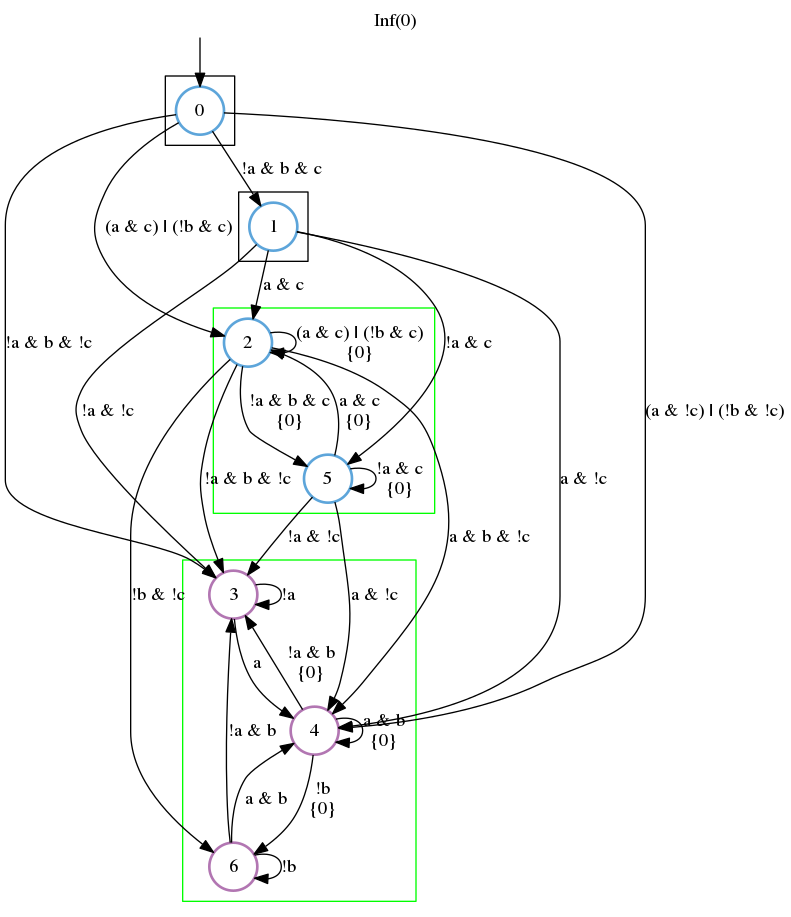
\includegraphics[scale=0.4]{img/highlight_language.png}
 \caption{An $\omega$-automaton colorized using \textbf{--hightlight-language} new option of
          \textbf{autfilt}}
 \label{fig:highlight_language}
\end{figure}

To come back to SAT-based minimization, by default, the binary search algorithm starts with 1 as
\textbf{min} value. Our theory is that the minimal automaton can not have less states than the total number
of languages recognized by each states. Instead of using 1 for \textbf{min} value, we set it to the total
number of recognized languages. This worked, it improved in general binary search algorithm but in somes
cases, which are far from negligible, the default binary search method was still better. This leads to a
new command line option: \textbf{sat-langmap}. This option is not set by default.%				All work details.
\chapter{Bibliography and glossary}
\printbibliography[heading=subbibliography]%			Bibliography and grossary.

\appendix
% Some configurations before appendix.

% Redefine the relevant code of \part command for Appendix.
\makeatletter
\renewcommand\part{%
  \if@openright
    \cleardoublepage
  \else
    \clearpage
  \fi
  \thispagestyle{empty}%	Original »plain« replaced by »emptyx.
  \pagenumbering{roman}%	Restart numbering in roman style.
  \if@twocolumn
    \onecolumn
    \@tempswatrue
  \else
    \@tempswafalse
  \fi
  \null\vfil
  \secdef\@part\@spart}
\makeatother

\part{Appendix}
\etocdepthtag.toc{mtappendix}
\etocsettagdepth{mtchapter}{none}
\etocsettagdepth{mtappendix}{subsection}
\etoctocstyle{1}{Contents (Appendix)}
\tableofcontents%		\part deredifinition and second table of contents.
\chapter{Company documentation}
\chapter{Hardware / Software Documentation}
\chapter{Gross results}
\end{document}
